\documentclass[a4j]{jarticle}

\usepackage[dvipdfmx]{graphicx}
\usepackage[dvipdfmx]{color}
\usepackage{epsbox}
\usepackage{url}
\usepackage{here}
\usepackage{ascmac}

\setlength{\headsep}{-5mm}
\setlength{\oddsidemargin}{0mm}
\setlength{\textwidth}{165mm}
\setlength{\textheight}{230mm}
\setlength{\footskip}{20mm}

\title{
\vspace{30mm}
{\bf システム提案書} 
\\
\vspace{5mm}
{\bf ZoologicAR \\園内AR案内アプリ}
\vspace{90mm}
}

\author{
\vspace{5mm}
Siesta \\
}

%date{
%平成29年4月17日
%}

\begin{document}
\maketitle

\newpage

\tableofcontents

\newpage

\section{はじめに}
近年では年々の入園者数が減少・大きな赤字など問題を抱えている動物園が多数存在しています.旭山市旭山動物園の入園者数を調べてみると年々減少傾向であることが確認できました(図~\ref{noichi},~\ref{noichi_akaji}参照)[1].高知県立のいち動物公園様でもこの問題を解決し入園者数を増やすことのできるような新たな提案を検討する必要があるという話を伺っております.そこで,私たちは新しい技術を用いたアプリケーションをご提案致します.これによりお客様に興味を持って頂くことで入園者数を増やすことが期待できます.

\begin{figure}[htb]
	\begin{center}
		\begin{tabular}{c}
			\begin{minipage}{0.5\hsize}
				\begin{center}
					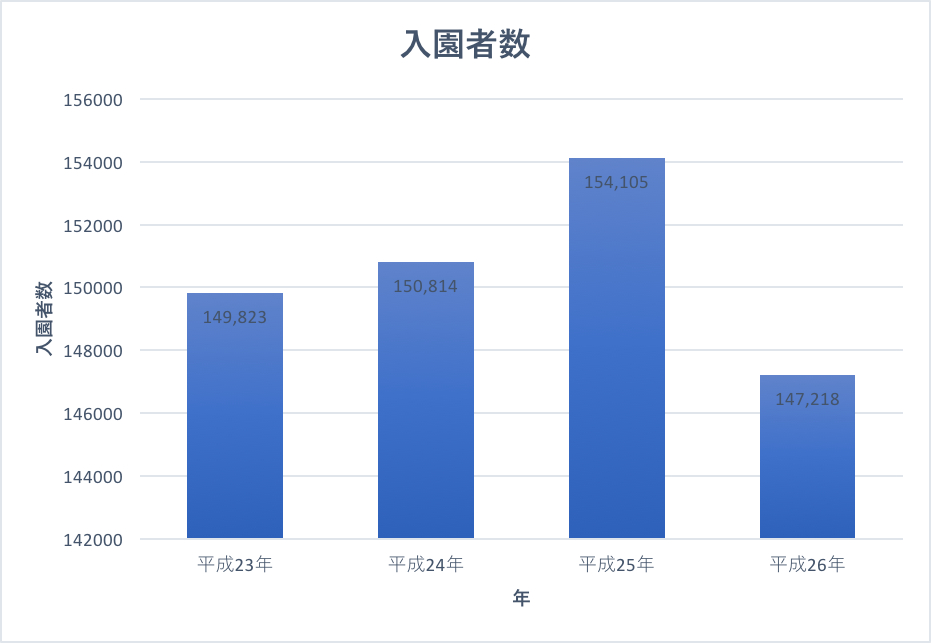
\includegraphics[width=0.6 \linewidth]{noichi.png}
					\caption{のいち動物公園の入園者数の遷移}
					\label{noichi}
				\end{center}
			\end{minipage}
			\begin{minipage}{0.5\hsize}
				\begin{center}
					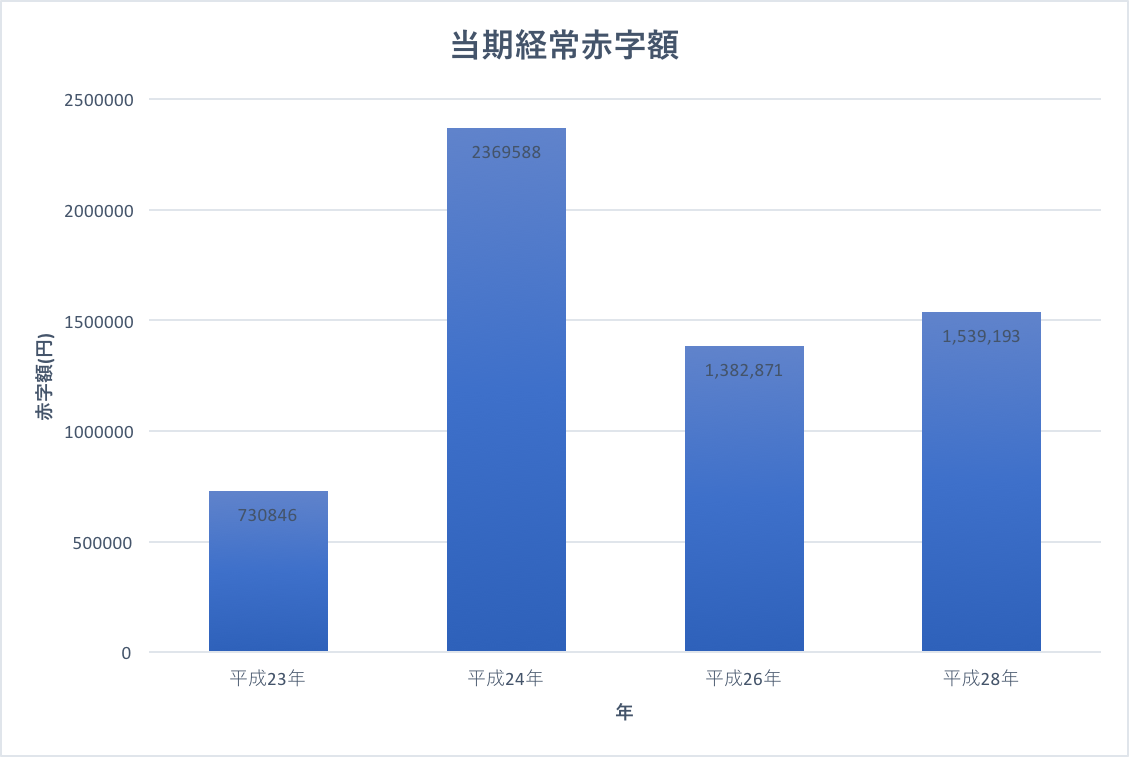
\includegraphics[width=0.6 \linewidth]{noichi_akaji.png}
					\caption{のいち動物公園の当期経常赤字額の遷移}
					\label{noichi_akaji}
				\end{center}
			\end{minipage}
		\end{tabular}
	\end{center}
\end{figure}


\section{解決できる課題}
現在,多数の動物園で入園者数が減少し,更に大きな赤字が出ているという現状があります.このような問題が発生している原因として,
\begin{itemize}
	\item 他の動物園との差別化が行えていない
	\item 子供が楽しめるようなシステムが少ないため,ファミリー層の入園者数が減少している
	\item リピーターが現れにくい
\end{itemize}
などが考えられます.

%また,動物園は公立施設とされているため比較的安価である入園料の値上げも難しいという現状もあります.


\section{課題解決のための提案}
本提案書では上記の課題を解決するものとして「園内AR案内アプリ(仮)」を提案します.

本システムでは以下のような機能を提供します.

\begin{itemize}
	\item 動物の情報を表示する機能
	%カメラで写した動物の…を画面内に表示します
	\item スタンプラリー機能
	%あるオブジェクトをスタンプとし,カメラで写すことにより獲得できるようにします
	\item 言語表示切替機能
	%日本語,英語,中国語に切り替えることができるようにします
	\item 園内マップ機能
	%園内のマップを表示します.また,設定した場所までの案内を行います.
	\item お手洗いの混雑状況確認機能
	%お手洗いの使用状況を表示し,混雑を緩和します.
\end{itemize}


\section{課題解決のための方法}
これらの機能を導入することで以下のような問題を解決することが見込まれます.

\begin{itemize}
	\item 動物の情報を表示する機能\\
	他の動物園との差別化を図る事により,宣伝性を高めることができます.
	\item スタンプラリー機能\\
	スタンプラリーを行い,子供達の興味を誘うことで家族での入園者を増やすことができます.
	\item 言語表示切替機能\\
	外国からの観光客でも使用可能にすることで入園者を増やすことができます.
	\item 園内マップ機能\\
	自身の現在地の表示を可能にさせることにより動物園の利便性を向上させ,イメージアップに繋げることができます.
	\item お手洗いの混雑状況確認機能\\
	お手洗いで混雑状況を確認することにより待ち時間を削減することができます.
\end{itemize}


\section{機能概要,前提条件,制約事項}

\subsection{機能概要}
\begin{enumerate}
	\item AR表示機能\\
	端末から動物を撮影することでその動物の詳細情報を画面上に表示します.画面には動物の名称を表示し,更にタップすることで詳細な説明画面へと遷移します.
	\item スタンプラリー機能\\
	隠されたQRコードを端末で読み込むことでスタンプを獲得できるようにします.
	\item 言語表示切替機能\\
	アプリケーションに表示される言語を英語,中国語に対応させ,外国人観光客でも本システムを利用しやすくします.
	\item 園内マップ機能\\
	園内のマップを表示します.また,現在地の表示を行います.
	\item 混雑状況確認機能\\
	カメラをトイレの入り口に設置します.また,撮影した静止画をサーバへ送信し,端末側から確認できるようにすることで混雑を緩和します.
	\item イベント通知機能\\
	動物園のイベント情報や新しい動物の情報などを通知します.
	%\item Liveカメラ機能\\
	%カメラを各動物が展示されている場所に設置します.本アプリケーションから動物のリアルタイムな映像を提供します.
\end{enumerate}

\subsection{前提条件}
本提案書では以下を前提条件としています.
\begin{itemize}
	\item 入場者が本システムの使用が可能な端末を所持していること
	\item 動物園がネットワーク環境下にあること
\end{itemize}

\subsection{制約事項}
本提案書では以下を制約条件としています.
\begin{itemize}
	\item 入場者が端末に本アプリケーションをインストールしていること
\end{itemize}

\section{情報の流れ}
このシステムは入力用PC,携帯端末,サーバ,Raspberry Pi,Webカメラより構成します.システム内部での情報の流れを図~\ref{data_nagare}に示します.

\begin{figure}[H]
	\begin{center}
		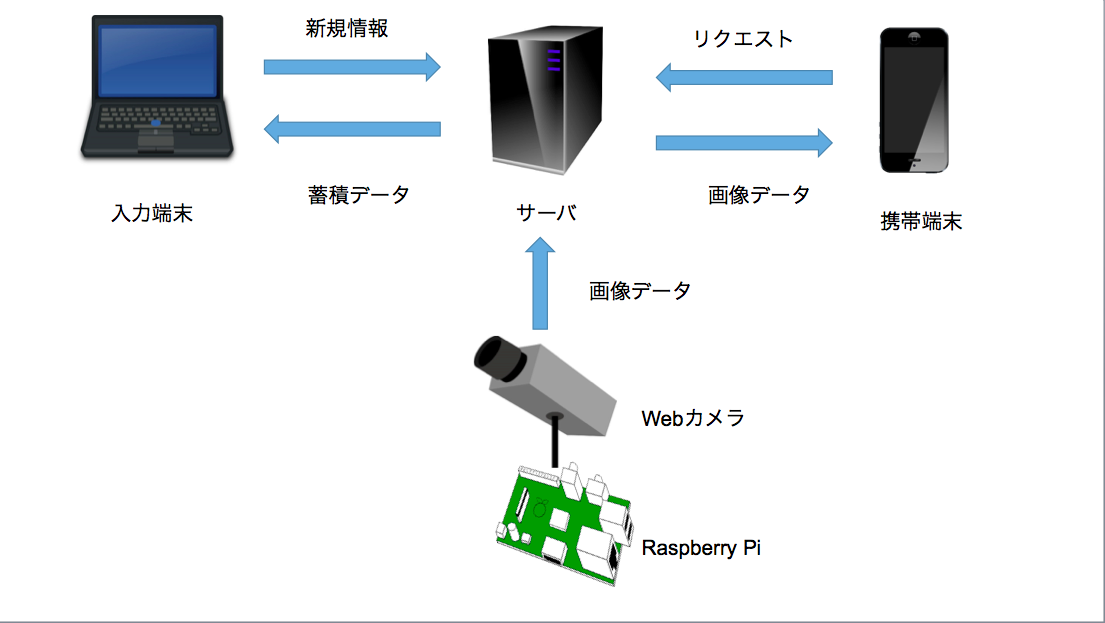
\includegraphics[width=0.8 \linewidth]{data_nagare_3.png}
		\caption{情報の流れ}
		\label{data_nagare}
	\end{center}
\end{figure}

利用者が撮影した画像をサーバに送信し,ARエンジンで画像認識を行います.認識して得た情報をもとに撮影した画像の情報を利用者端末に送信をします.

Webカメラで撮影した映像をサーバに送信し,サーバから利用者端末に送信します.

\section{システムインターフェース}
システム間のやりとりは安全に行うためにHTTPS通信を用いて行います.

\section{想定する利用者}
本システムを利用するものは以下の通りです.
\begin{itemize}
	\item 動物園の従業員
	\item 動物園の利用者
\end{itemize}

\section{システムのハードウェア構成}
システムのハードウェア構成は表\ref{hardware}の通りです.

\begin{table}[H]
	\caption{ハードウェア構成}
	\begin{center}
 	  \begin{tabular}{|c|c|}\hline
            		項目 & 数量 \\ \hline
			入力用PC & 1台 \\ \hline
			携帯端末 & 1台 \\ \hline
			サーバ用PC & 1台 \\ \hline
			Raspberry~Pi & 3台 \\ \hline
			Webカメラ & 3台\\ \hline
		\end{tabular}
		\label{hardware}
	\end{center}
\end{table}


%ソフトウェアはwikitude(画像認識),MySQL(データベース)を用いて構成します.また,使用する言語はjavascript(HTML内の一部のプログラム),SQL(データベース),HTML(ホームページ),CSS(ホームページ)を用いて構成します.

\section{導入・移行計画}
2017年2月5日をもって,システムの導入を完了します.

\section{保守・運用}
提案システムを以下のように保守・運用します.

\begin{enumerate}
	\item 運用は動物園の管理者が情報の更新を行います.
	\item 故障発生時は弊社にて対応させていただきます.
\end{enumerate}

\section{作業標準}
システム開発にかかる作業標準は貴社ご指定のものを使用します.

\section{品質管理}
システム開発にかかる品質管理手法は貴社ご指定のものを使用します.

\section{工程計画}
工程計画は次の通りです.\\

要求分析完了:2017年10月26日

外部設計完了:2017年11月27日

内部設計完了:2017年12月18日

開発完了:2018年1月25日

導入:2018年2月5日

\section{体制}
このシステムの開発は弊社の8名のエンジニアにより実施します


\section{システム化にかかる費用とその効果}
システム化にかかる費用の概算は次の通りです.
\begin{table}[H]
  \caption{システム化にかかる費用}
  \begin{center}
    \begin{tabular}{|c|c|c|c|c|} \hline
      項目&単価(円)&数量&金額(円)&備考 \\ \hline
      Raspberry~pi&6,000&3台&18,000& \\ \hline
      Webカメラ&4,000&3台&12,000& \\ \hline
      サーバ用PC&150,000&1台&150,000& \\ \hline
      システム開発人件費&15,000&480日&7,200,000&工数内訳 8人×60日 \\ \hline
      \multicolumn{3}{|c|}{開発費}&7,380,000&上記4つの合計 \\ \hline
      \multicolumn{3}{|c|}{維持費}&3,690,000&減価償却期間×開発費×10\% \\ \hline %減価償却期間×開発費×0.15
      \multicolumn{3}{|c|}{総コスト}&11,070,000&開発費+維持費 \\ \hline
    \end{tabular}
  \end{center}
\end{table}
本システムを実現させた場合,導入年から5年間で動物園入園者が40\%増加すると想定して試算を行います.
現在の年間有料入園者数を最新の入園者データから5.2万人とした場合,本システムを導入することによって増加する動物園の利益は
\begin{screen}
  \begin{center}
    460(入園料)×52,000(現在の年間有料入園者数の人数)×0.4(入園者の想定増加割合) = 9,568,000円
  \end{center}
\end{screen}
となります.
また,入園者の増加分だけ園内の飲食施設の利用者数が増加することを考慮します.
現在の年間入園者数を最新の入園者データ[2][3]から17万人とした場合,自販機でのドリンク購入やレストランにおいての利益の1人あたり平均を40円とした場合の増加する動物園の利益は
\begin{screen}
170,000(入園者の人数)×0.4(入園者の想定増加割合)×40(1人あたり増加する動物園の利益) = 2,720,000円
\end{screen}
となります.
以上のことから,開発側の経営利益は
\begin{screen}
\begin{center}
9,568,000(増加人数分の入園料の利益) + 2,720,000(レストランからの利益) - 11,070,000(総コスト)
\end{center}
\begin{flushright}
=1,218,000円
\end{flushright}
\end{screen}
と見積もることができます.
\section{本システム提案のアピールポイント}
本システム提案におけるアピールポイントについて説明します.
\begin{description}
\item[(1)  ] 動物園入園者に対して,動物園を楽しんで頂くための園内AR案内アプリ(仮)です.入園者に携帯端末のアプリケーションを用いて楽しんで頂くという点で他の動物園との差別化を可能にします.
\item[(2)  ] アプリの機能を用いて,現在地をマップで表示することで,入園者が園内の状況を把握できるようにします.
\item[(3)  ] 本アプリケーションは,英語,中国語に対応しているため,外国人入園者の方でも動物園をお楽しみ頂けます.
%\item[(4)] スタンプラリー完成時に動物園のグッズのプレゼントなどを行うことでお子様でも動物園を存分にお楽しみ頂けます.
\item[(4)  ] 園内のイベント情報や新たな動物加入の情報を通知することで園内の変化を利用者に知らせます.そうすることでリピーターの増加が見込まれます.
\item[(5)  ] (1),(2),(3),(4)のような多様な機能を実現させることによって,動物園のイメージアップが見込まれます.その結果,動物園の入園者の増加が見込まれます.
\end{description}

\section{用語の定義}
  本提案書では,次の通りに用語を定義します.
\begin{itemize}
\item Raspberry~Pi:ARMプロセッサを搭載したシングルポート・コンピュータ
\item AR:Augmented~Reality(拡張現実)の略称.現実世界の映像に対し,位置情報などのデータや実際に存在しない情報をCGと重ねて表示させる手法.
%\item wikitude:携帯端末のARアプリを開発できるプログラミングソフトウェア.
%\item MySQL:オープンソースのデータベース管理システム.
%\item javascript:プログラミング言語の一つであり,主に動的なウェブサイト構築やウェブアプリケーション開発の際に用いられる.
%\item HTML:Hyper~Text~Markup~Languageの略で,ウェブページを作成するためのプログラミング言語である.インターネット上のウェブページの殆どはHTMLで作成されている.
%\item CSS:Cascading~Style~Sheetsの略で,ウェブページのスタイルを指定するための言語である.HTMLと組み合わせて使用される.
\end{itemize}

\bibliographystyle{jplain}
\begin{thebibliography}{9}
\bibitem{ref1}
高知県立のいち動物園, \url{http://www.noichizoo.or.jp/}, 2017年10月13日アクセス  
\bibitem{ref2}
  高知県のいち動物公園協会 業務に関する資料, \url{http://www.noichizoo.or.jp/noichi_hp/gyoumu.html}, 2017年10月13日アクセス

\end{thebibliography}

\end{document}

